\documentclass[pdftex, 11pt, a4paper, titlepage]{article}

\usepackage[utf8]{inputenc}
\usepackage[T1]{fontenc}
\usepackage[french]{babel}
\usepackage{fullpage}
\usepackage{color}
\usepackage{url}
\usepackage{wrapfig}
\usepackage{alltt}
\usepackage{listings}
\usepackage{fixltx2e}
\usepackage{graphicx}
\usepackage{caption}
\usepackage{subcaption}
\usepackage{mathtools}
\usepackage{amsmath}
\usepackage[hidelinks]{hyperref}
\frenchspacing
\setlength{\parskip}{0.0em}
\setlength{\parindent}{0.0em}
\setcounter{secnumdepth}{0}
\tolerance=1000
\newcommand{\vect}[1]{\overrightarrow{#1}}

\begin{document}
\title{Rendu de scène sous OpenGL}
\author{Nabil Boutemeur,
         Cassian Assael,
   Alessandro Bonnafous} 
\date{Octobre 2014}
\maketitle

\setcounter{tocdepth}{4}
\setcounter{secnumdepth}{-1}

\tableofcontents
\setlength{\parskip}{0.5em}
\pagebreak

\begin{abstract}
  Le but du projet est de fournir une démonstration de principes
  mathématiques appliqués à un programme, et en même temps, montrer
  l'application d'objets mathématiques tels que les matrices et les
  vecteurs en vrai, car bon nombre de concepts sont applicables dans
  la réalité.

  Nous voulons donc écrire un programme qui montre les trois
  transformations de base possibles dans l'univers 3D:
  \begin{itemize}
  \item Translation
  \item Rotation
  \item Homothétie
  \end{itemize}
\end{abstract}
\pagebreak
\section*{Mise en oeuvre}

Après concertation, nous nous sommes décidés à faire une scène
montrant trois objets avec des formes (plus ou moins) primitives.
Chacun de ces objets est ``activable'' à partir d'une touche de
clavier, et provoquant pour chacun, l'animation d'une transformation.

\section*{Outils utilisés}

Nous utilisons l'outil \textbf{git} comme logiciel de gestion de
version, il permet de mieux repérer les régressions introduites au fil
de la modification du code, et facilite le travail collaboratif, car
chaque modification du code est associé a son auteur.

Le dépôt est disponible en libre accès sur
\href{https://github.com/nbouteme/OpenGL-Demo}{{\color{blue}Github}}
\footnote{\url{https://github.com/nbouteme/OpenGL-Demo}},
sous license LGPLv3.  \textbf{Github} étend l'aspect collaboratif de
git en fournissant un ensemble de service lié à un dépôt.

Cela comprend notamment le service d'intégration continue
\href{https://travis-ci.org/nbouteme/OpenGL-Demo}{{\color{blue}Travis}}
\footnote{\url{https://travis-ci.org/nbouteme/OpenGL-Demo}},
qui, lorsqu'un changement se produit sur le dépôt va régénérer un
environnement de développement et recompiler le projet, pour s'assurer
que le code sur le dépôt principal sera toujours prêt à être déployé.

Il va aussi s'assurer que, lorsqu'un tiers veut contribuer du code au
dépôt, la fusion du code existant et du code en attente d'intégration
soit toujours fonctionnel.

Concernant le programme lui-même, nous utilisons \textbf{cmake} comme
système de build, le but du système de build étant de correctement
lier entre elle les différentes partie du projet et s'assurer que
toutes les dépendances sont satisfaites. Le programme cmake génère
alors un makefile qui reconstruit les cibles dont au moins une
dépendance aura été modifiée. La puissance de cmake réside aussi dans
le fait qu'il n'est pas limité à générer des makefile, mais aussi des
fichiers de projet pour la plupart des IDE. Cela permet aux
collaborateurs d'utiliser leur outil de choix pour modifier le code.

Ensuite, le programme utilise la version 3.3 du standard
\textbf{OpenGL}.  Nous avons choisi cette version en particulier car
c'est la version la plus répandue à l'heure actuelle. Elle a introduit
des changements majeurs dans l'API OpenGL ainsi que supprimée des
fonctionnalités considérées comme néfaste pour un projet
\footnote{\url{https://www.opengl.org/wiki/Legacy_OpenGL}}

Nous utilisons la bibliothèque \textbf{GLEW}, qui permet de charger à
l'exécution du programme les fonctions OpenGL supportée par le pilote
graphique, ainsi qu'éventuellement des extensions du standard, la
bibliothèque \textbf{GLM} qui fournit une API permettant de manipuler
certains types primitifs disponibles dans le langage de programmation
de shader \textbf{GLSL}, notamment les matrices et les vecteurs. La
bibliothèque \textbf{SOIL} qui est une bibliothèque C très légère,
permettant le chargement et la décompression de format d'images. Et
pour finir, la bibliothèque \textbf{GLFW}, elle aussi minimaliste, qui
gère les entrées et les sorties du programme --- Fenêtre, souris,
clavier, manette --- en plus de la création du contexte OpenGL.

Nous utilisons aussi \href{https://nbouteme.github.io/OpenGL-Demo/docs}{{\color{blue}Doxygen}}
\footnote{\url{https://nbouteme.github.io/OpenGL-Demo/docs}},
 pour générer la documentation.

\pagebreak

\part{Conception du programme}

\section{Squelette du programme}

Cette section ne décrit que les classes du programme en surface.

\subsection{Singleton --- Classe \texttt{Application}}

Le but du singleton ici est de gérer un ensemble de ressources unique
au programme.  Il est identique au singleton de Meyers, si ce n'est
qu'un pointeur de fonction est utilisé pour récupérer son instance, au
lieu de vérifier à chaque appel si le singleton a déjà été instancié.

La fenêtre à afficher hérite d'une classe d'interface, pour
modulariser le singleton et pouvoir instancier des fenêtres utilisant
une autre API qu'OpenGL.

\subsection{Fenêtre --- Classe \texttt{GLWindow}}

Dans son constructeur, la fenêtre se contente d'appeler des fonctions
d'initialisation OpenGL et GLFW. Puis la méthode run, s'occupe de
gérer la boucle principale, en créant une scène, et en l'affichant.

\subsection{Scène --- Classe \texttt{Scene}}

Une scène est un agrégat d'objets pouvant être dessinés, et pouvant
être mis à jour (update) en plus d'une caméra.  Elle peut aussi
contenir un ensemble d'effets de post-processing. On ne peut pas
instancier une scène telle quelle, la classe doit être dérivée,
puis les objets qu'elle doit afficher sont instanciés dans son
constructeur.

\subsection{Modèles --- Classe \texttt{Model}}

Un modèle est un ensemble de faces, dont chaque sommet possède des
attributs --- Normales et coordonnées de texture ---.  Dans le projet,
un modèle est donc une figure géométrique \textbf{simple}

Il est intéressant de noter que j'emploie le terme \textbf{normale},
ici, avec le terme \textbf{sommet}, alors qu'une normale est un
vecteur dénotant une direction perpendiculaire à une
\textbf{face}. C'est parce que chaque sommet faisant partie d'un modèle
peut faire partie de plusieurs faces, et on doit donc utiliser une
normale différente pour un même sommet dans le traitement d'une face
distincte.Lorsque des normales ne sont pas utilisées, la classe \texttt{Model}
accepte un tableau d'éléments, en plus d'un tableau de sommets. Le
tableau d'éléments permettra alors de réutiliser des points déjà
définis en utilisant leur indices, économisant ainsi de la VRAM et de
la bande passante.Dans la pratique, le tableau d'élément n'est jamais utilisé, car nous
avons besoin des normales pour des applications plus intéressantes,
notamment dans l'éclairage, d'ailleurs, un des avantages des normales
est que l'on peut avoir des normales qui ne correspondent pas vraiment
a la perpendiculaire d'une face, permettant en quelque sorte de
tromper les calculs de lumière, et ainsi montrer plus de détail qu'il
y en a vraiment.

La classe \texttt{Model} n'est pas instanciable d'elle même, il faut
la dériver pour pourvoir l'utiliser.

\pagebreak
\subsection{Fichiers OBJ --- Classe \texttt{OBJData}}

La classe \texttt{OBJData} fait une analyse de la syntaxe du code qui
lui a été fourni, et construit alors un tableau de sommet/attribut
prêt à l'emploi pour une utilisation dans l'API OpenGL.

Du fait de la définition précédente de ``Modèle'' comme étant une
figure géométrique simple, \texttt{OBJData} a été conçu seulement pour
lire des fichiers \texttt{OBJ} basique.

Un fichier \texttt{OBJ} est défini par, dans l'ordre:
\begin{itemize}

\item une liste de sommets, tous séparés par un retour à la ligne:
  \begin{alltt}
    v \emph{x} \emph{y} \emph{z}
  \end{alltt}
  Où x, y et z sont des nombres à virgules flottantes.

\item une liste optionnelle de coordonnées de texture, toutes séparées
  par un retour à la ligne:
  \begin{alltt}
    vt \emph{u} \emph{v}
  \end{alltt}
  Où u et v sont des nombres à virgules flottantes.

\item une liste optionnelle de normales, toutes séparées par un retour
  à la ligne:
  \begin{alltt}
    vn \emph{x} \emph{y} \emph{z}
  \end{alltt}
  Où x, y et z sont des nombres à virgules flottantes.

\item une liste de faces, toutes séparées par un retour à la ligne:
  \begin{alltt}
    f
    \emph{x\textsubscript{1}}/\emph{y\textsubscript{1}}/\emph{z\textsubscript{1}}
    \emph{x\textsubscript{2}}/\emph{y\textsubscript{2}}/\emph{z\textsubscript{2}}
    \emph{x\textsubscript{3}}/\emph{y\textsubscript{3}}/\emph{z\textsubscript{3}}
  \end{alltt}
  Où x\textsubscript{n}, y\textsubscript{n} et z\textsubscript{n} sont
  les indices des déclaration des Sommet/Coordonnées de
  texture/Normale et n
  le sommet constituant la face --- OpenGL, et par extension OBJData, veulent
trois points par face.
\end{itemize}

Par exemple, un triangle rectangle, avec une seule normale
perpendiculaire serait défini par le fichier suivant, prenant en
compte trois définitions possibles d'une face:
\begin{alltt}
v 0.000000 1.000000 0.000000 
v 1.000000 0.000000 0.000000
v 1.000000 1.000000 0.000000
vt 0.000000 1.000000
vt 1.000000 0.000000
vt 0.000000 0.000000 
vn 0.000000 0.000000 1.000000
f 1/1/1 2/2/1 3/3/1 # tout les attributs 
f 1/1 2/2 3/3       # sommet et textures
f 1//1 2//1 3//1    # sommet et normales
\end{alltt}

\pagebreak
\subsection{Caméra --- Classe \texttt{Camera}}

La caméra est une simple classe qui se contente de garder avec elle la
matrice de vue et de projection, et gérer les entrées au
clavier/souris/manette.

\subsection{Shader --- Classe \texttt{Shader}}

Un shader est un programme exécuté à divers niveaux de la pipeline
graphique du GPU.  Ils ont l'avantage d'être très flexible, et surtout
très puissant, car il bénéficient de la puissance de calcul parallèle
monstrueuse du GPU.

Un shader n'est pas lié à un modèle en particulier, mais ils est
simplement utilisé par OpenGL lorsqu'il effectue du dessin dans un
tampon.

Un shader est le résultat de la compilation d'au moins 2 programmes de
base, le vertex shader, qui effectue des calculs sommet par sommet,
notamment pour effectuer des transformation, selon les paramètres
qu'il lui auront été passé avant le dessin, et le pixel shader, qui va
donner une couleur à un pixel en fonction des paramètres qui lui
auront été donnés avant le dessin, ou récupérés directement du vertex
shader, qui s'exécute avant le pixel shader dans la pipeline.

Il existe aussi des geometry shaders, qui permettent notamment de
générer de manière procédurale des objets tridimensionnels, et --- à
partir d'OpenGL 4.0 --- les compute shaders qui sont utilisé pour des
calculs plus généraux, comme par exemple des simulations d'évènements
physiques comme des tissus, et le couple Tesselation
Control/Evaluation shader qui prend une géométrie existante, en génère
des sommets puis applique à ces nouveau sommets des transformations
supplémentaire, ils sont surtout utilisé pour augmenter le niveau de
détail d'un objet.

La classe \texttt{Shader} s'occupe donc de la vie d'un shader, de sa
création à sa destruction.  Elle combine un vertex shader et un
fragment shader, et accessoirement un geometry shader, et les combine
en un seul shader prêt a l'emploi.

\subsubsection{Exemple de vertex shader basique}
Voici un exemple de vertex shader qui se content d'effectuer la
transformation d'un sommet, de son espace-local en coordonnées écran.

\begin{lstlisting}
#version 330 core
layout (location = 0) in vec3 pos;
uniform mat4 proj;
uniform mat4 view;
uniform mat4 model;

void main()
{
  gl_Position = proj * view * model * vec4(pos, 1.0);
}
\end{lstlisting}
\pagebreak
\subsubsection{Exemple de fragment shader basique}
Ce shader se contente de colorer en blanc les pixels qui sont affiché
durant un dessin.

\begin{lstlisting}
#version 330 core
out vec4 outColor;

void main()
{
  outColor = vec4(1.0f);
}
\end{lstlisting}

\subsection{Effet --- Classe \texttt{Effect}}

La classe \texttt{Effect} représente un effet de post-processing appliqué à
une scène, qui peut elle contenir plusieurs effets.
Lors du rendu, la scène est dessinée dans un tampon, qui lui ne sera pas
affiché, mais seulement dessiné dans une texture. Puis cette texture
sera dessinée dans un rectangle qui couvre tout l'écran, avec un shader
qui effectura un traitement pixel par pixel. C'est le post processing.
La classe \texttt{Effect} propose 2 effets par défaut, une inversion de couleur,
et un flou progressif (l'image se floute progressivement sur les bords)

\subsection{Gestion des ressources}

Un des problèmes qui s'est posé pendant le développement était :
comment est-ce que tout ces modèles, shader, texture, etc, allais être
chargé dans le programme ?  Est-ce que les garder dans un fichier
était la solution idéale ? Le programme serait contraint de se
trouver dans un répertoire à partir d'où il avait accès à toutes ses
ressources, avec les bonnes permissions, et un déplacement ou une
copie de l'exécutable s'accompagne de tout ses fichiers.  Une première
solution avait était d'utiliser le linker ld, qui est capable de
transformer n'importe quel fichier en .o, pouvant être linker
statiquement dans le programme, cela posait trois autre problèmes, le
nom de symboles généré par ld n'était pas paramétrable, et donnait
trois symboles sous la forme ``\_binary\_\textit{nom}\_\textit{extension}\_''
 suivis de \texttt{start}, \texttt{end}, et \texttt{size}. Ensuite 
le problème était que pour chaque fichier ajouté, il fallait ajouter
 trois symboles au code du programme, et c'est vite devenu pénible 
à gérer, et dernièrement, le symbole censé représenter la taille, 
ne contenait pas vraiment la taille, mais son adresse elle même 
était la taille d'une ressource.

Au final, un format de fichier RES d'archivage sans compression a été
conçu pour répondre à ce besoin, ainsi qu'une classe capable de
manipuler ce type de fichier, situé dans une bibliothèque séparée et
un exécutable génère les archives, et ld n'a plus qu'à linker ces
archives avec l'exécutable final, nécessitant alors seulement de
modifier le code du programme non plus à chaque ajout de fichier, mais
à chaque ajout de répertoire, ce qui n'arrive pas souvent.

\pagebreak

\section{Format fichier RES}

Le header d'un fichier RES défini de la manière suivante.

Le header commence par les 3 caractères ASCII ``RES'' suivi d'un octet
présentant la version du format d'archive --- typiquement 1 --- suivi
du nombre de ressource contenue dans le ficher, encodé en big endian,
sur 32 bits.  Une archive valide vide a donc une taille de 8 octets.

Ensuite le header contient une table de ressource, de taille variable,
car chacune de ses entrées a une taille variable.  Une entrée dans la
table est typiquement la suivante, en format hexadécimal:

\begin{alltt}
[ aa aa aa aa ] [ bb {... a fois ...} bb]
[ cc cc cc cc] [ dd dd dd dd ]
\end{alltt}

Où \textbf{aa aa aa aa} est un entier 32 bits non signé en big endian
représentant la taille du nom de la ressource, \textbf{bb ... bb} est
le nom de la ressource, \textbf{cc cc cc cc} est un entier 32 bits non
signé en big endian représentant la taille de la ressource elle même,
et enfin \textbf{dd dd dd dd} est un entier 32 bits non signé en big
endian représentant l'adresse du premier octet de la ressource dans
l'archive.

Enfin, le header est constitué d'octets à 0 jusqu'à être aligné avec
le segment qui suit --- padding.

\section{Gestionnaire de Ressources --- Classe
  \texttt{ResourceManager}}

La classe \texttt{ResourceManager} s'en tient au spécifications
données précédemment pour permettre de lire, gérer et sauvegarder une
archive.

\section{Générateur de Ressources --- Programme \texttt{resgen}}

Le programme \texttt{resgen} prend une liste de fichiers en paramètre,
et en créer une archive, écrite sur la sortie standard.  Si un des
fichier est une archive RES, alors elle n'est pas ajouter à l'archive
en cours de création mais ses ressources le sont.  Comme l'archive
résultante est ecrite sur la sortie standard, vous sauvegarder une
archive <<The Unix Way>>, avec la redirection de votre shell:
 
\begin{alltt}
\$> ./resgen file1 file2 > ar.res
\end{alltt}

\section{Utilisation de la ``nouvelle'' API d'OpenGL}

Ce qui a causé la création du Core Profile d'OpenGL fut en parti due à
la popularité de la programmation orientée objets.  En effet,
l'ancienne API d'OpenGL était très procédurale, les programmes n'était
constitué que de grandes listes d'appels à des fonctions, sans
structure.

Le Core Profile introduit les \textbf{objets} OpenGL, ainsi que des
fonctions permettant de les manipuler. Cela a rendu l'encapsulation dans
des classes de langages de plus haut niveau plus simple.

Notre programme en utilise quelques uns, leur fonctionnement est
détaillé dans cette section.

\subsection{Modèles}

Avec OpenGL 3.3, l'utilisation des Vertex Array Objects est devenu
obligatoire, avec les Vertex Buffer Objects.  Notre classe Model
utilise ces deux types d'objets, ainsi que des Element Buffer Object
si nécessaire.

\subsubsection{Vertex Array Objects}

Un Vertex Array Object (\emph{VAO}) est un objet qui conserve en mémoire les
attributs et leur format d'un tampon.  Imaginez un ensemble de données
qui contient les uns à la suite des autres, des données pour chaque
sommets d'un objet:

Pour créer un \emph{VAO}, vous générez un tampon, puis vous l'activez de
cette manière:

\begin{lstlisting}
int vao;
glGenVertexArrays(1, &vao); glBindVertexArray(vao);
\end{lstlisting}


\begin{alltt}
[x y z u v a b c][x y z u v a b c]...[x y z u v a b c]
\end{alltt}
Où les [ ] dénotent un sommet x, y et z sont sa position, u et v des
coordonnées de texture, et a b c, une normale.

Le VAO lui, défini comment ces attributs sont dans la mémoire de la
manière suivante:

\emph{Les coordonnées de sommets sont constitués de 3 nombres, la
  distance entre les coordonnées de sommets de 2 points est de 8
  nombres\\}
\emph{Les coordonnées de texture sont constitués de 2
  nombres, après avoir sauter 3 nombres, la distance entre les
  coordonnées de texture de 2 points est de 8 nombres\\}
\emph{Les normales sont constitués de 2 nombres, après avoir sauter
 5 nombres, la distance entre les normales de 2 points est de 8
 nombres\\}

Le \emph{VAO} défini aussi où, dans le vertex shader, ces données seront
placés.  Le programmeur définit ces informations une seule fois avec
les appels OpenGL, et le \emph{VAO} se contentes de les enregistrer et de le
redonner quand nécessaire:

\begin{lstlisting}
// location 0 du vertex shader
// 3 float
// sizeof float (4) * distance entre sommets (8) = 32

// sauter 0 nombres
glVertexAttribPointer(0, 3, GL_FLOAT, false, 32, nullptr);
glEnableVertexAttribArray(0);

// sauter sizeof float (4) * 3 nombres = 12
glVertexAttribPointer(1, 2, GL_FLOAT, false, 32, (void *)12);
glEnableVertexAttribArray(1);

// sauter sizeof float (4) * 5 nombres = 20 
glVertexAttribPointer(2, 3, GL_FLOAT, false, 32, (void *)20);
glEnableVertexAttribArray(2);
\end{lstlisting}

Notez que l'ensemble de données est défini de manière implicite, ici,
vous devez le générer et l'activer avant de faire des appels à
\texttt{glVertexAttribPointer}.

Maintenant, où sont stockés ces ensembles de données ?

\subsubsection{Vertex Buffer Object}

Un Vertex Buffer Object (\emph{VBO}) se contente typiquement de garder de
l'information relative à un objet que vous voulez afficher, tel que
les sommets, normales, mais vous pouvez y mettre ce que vous voulez
tant que vous êtes organisé.

Pour créer et activer un \emph{VBO}, ça se passe quasiment comme pour les
VAO:

\begin{lstlisting}
glGenBuffers(1, &vbo);
glBindBuffer(GL_ARRAY_BUFFER, vbo);
\end{lstlisting}

Le \texttt{GL\_ARRAY\_BUFFER} est une ``cible'', c'est ici que vous
voulez garder en mémoire vos sommets.

Ensuite, vous voulez remplir votre buffer,

\begin{lstlisting}
glBufferData(GL_ARRAY_BUFFER,
             size * sizeof(float),
             ptr, GL_STATIC_DRAW);
\end{lstlisting}

Où \textit{size} est le nombre de données que vous multipliez par la taille
d'une seule données, pour avoir le nombre d'octets à copier, à partir
du pointeur ptr.  \texttt{GL\_STATIC\_DRAW} indique à OpenGL qu'on ne
viendra pas plus tard modifier ces données, puisque on se contente de
les afficher et d'effectuer des transformations dessus.
Maintenant, quand on veut dessiner un objet, on bind le \emph{VAO}, active le
shader, et on dessine:

\begin{lstlisting}
glBindVertexArray(vao);
glUseProgram(shader);
...
glDrawArrays(GL_TRIANGLES, 0, nbSommets);
\end{lstlisting}

\pagebreak
\subsubsection{Element Buffer Object}

Vous avez sûrement remarqué que quand on veut dessiner un objet, on
utilise des triangles.  Un triangle a trois sommets.

Maintenant, supposons que l'on veuille dessiner un carré. Eh bien on
ne peut pas le faire avec 4 sommets, On doit dessiner deux triangles
rectangle avec 2 points en communs. Ce qui fait 6 points.

C'est là que les \emph{EBO} interviennent. Au lieu de définir 6 points, et de
dessiner 2 triangles, vous définissez 4 points, et vous dessinez 2
triangles en réutilisant leur indices. Un peu comme le fait le format
OBJ.

\begin{lstlisting}
glGenBuffers(1, &ebo);
glBindBuffer(GL_ELEMENT_ARRAY_BUFFER, ebo);
glBufferData(GL_ELEMENT_ARRAY_BUFFER,
             size * sizeof(int),
             ptr,
             GL_STATIC_DRAW);
\end{lstlisting}

Maintenant, supposons un \emph{VBO} contenant 4 points:
\begin{verbatim}
0.000000 0.000000 0.000000
0.000000 1.000000 0.000000
1.000000 0.000000 0.000000
1.000000 1.000000 0.000000
\end{verbatim}

On peut alors dessiner un carré avec un EBO contenant

\begin{verbatim}
0 1 2 2 1 3
\end{verbatim}

Avec
\begin{lstlisting}
glBindVertexArray(vao);
glUseProgram(shader);
 ...
glDrawElements(GL_TRIANGLES, n, GL_UNSIGNED_INT, 0);
\end{lstlisting}

Où \textbf{n} est le nombre de sommets à dessiner.

Le gros désavantage de cette méthode est que vous êtes restreint à un
seul attribut par point, quel que soit la face. Pour des normales par
exemple, soit vous les recalculer, soit vous vous passez des \emph{EBO}.

\pagebreak

\subsection{Shaders}

Les shaders étant des programmes exécutés sur le GPU, ils utilisent un
langage particulier conçu pour cet usage, le \textbf{GLSL}.

Le GLSL est un langage dérivé du C, mais même si il bénéficie de type
primitifs plus évolué qu'en C, il reste un peu moins flexible (pas de
pointeur, pas d'allocation dynamique...)

Le shader est le programme compilé qui est exécuté sur le GPU au
moment du dessin, il est donc important de l'activer (bind) juste
avant un appel à \emph{glDrawArrays}.

Pour créer un shader, on compile les différent stades de la pipeline
(vertex et fragment), pour cela, vous donnez à OpenGL le code source
des shaders.
\begin{lstlisting}
  glShaderSource(vsID, 1, &vs, nullptr);
  glShaderSource(fsID, 1, &fs, nullptr);
\end{lstlisting}

Ensuite vous les compiler.

\begin{lstlisting}
glCompileShader(vsID);
glCompileShader(fsID);
\end{lstlisting}

On indique à quel programme ces shaders sont associés.

\begin{lstlisting}
glAttachShader(shaderID, vsID);
glAttachShader(shaderID, fsID);
\end{lstlisting}

Avant de link ces programmes en un seul, on donne le nom de la
variable qui contient la sortie de la pipeline (la couleur) avec
\texttt{glBindFragDataLocation}

\begin{lstlisting}
glBindFragDataLocation(shaderID, 0, ``outColor'')
\end{lstlisting}

Vous pouvez passer des paramètres à votre shader à travers des
\emph{uniform}, les \emph{uniform} sont des valeurs constantes 
dans un shader durant tout le temps de l'exécution d'un shader,
 (lisez, un appel à \texttt{glDraw*}),le mot clé \emph{uniform} 
est appelé un \textit{qualifier}

Vous déclarez un \emph{uniform} dans votre programme avec le mots clé
\emph{uniform}, puis selon son type, (float, vec, mat...), OpenGL vous fourni
divers manière d'uploader ces valeurs à votre shader.

Par exemple, pour des matrice 4x4, vous avez
\texttt{glUniformMatrix4fv}.  Notez que pour utiliser ces fonctions
vous devez obtenir un nombre qui sert de référence à votre uniform,
pour qu'OpenGL sache où mettre les données que vous lui donnez. Pour
cela on utilise \texttt{glGetUniformLocation}.

\begin{lstlisting}
uM = glGetUniformLocation(shaderID, "model");
...
glUniformMatrix4fv(uM, 1, GL_FALSE, value_ptr(M));
\end{lstlisting}
\pagebreak
\subsubsection{Transformations}

De base, nous avons besoin d'appliquer des transformations à des
sommets situé dans un espace local à l'objet.  Pour cela, nous
utilisons des matrices de transformation.  En multipliant une matrice
de modèle par les sommets du modèle, plus une composante w, qui
traduit les coordonnées d'espace local en espace monde.

La matrice de modèle définit les transformations de base à appliquer,
Translation, rotation, homothétie.  De base, la matrice de modèle est
une matrice identité

Pour définir les transformations, on multiplie cette matrice identité
par des matrices de Translation.

\begin{equation*}
M_{translation} =
  \begin{bmatrix}
    1 & 0 & 0 & \color{red}{T_x} \\
    0 & 1 & 0 & \color{green}{T_y} \\
    0 & 0 & 1 & \color{blue}{T_z} \\
    0 & 0 & 0 & 1
polyte  \end{bmatrix}
\end{equation*}

Où \emph{T} est un vecteur tridimensionnel définissant la translation

Pour l'homothétie :

\begin{equation*}
  M_{homothetie} =
  \begin{bmatrix}
    \color{red}{S_x} & 0                  & 0                 & 0 \\
    0                & \color{green}{S_y} & 0                 & 0 \\
    0                & 0                  & \color{blue}{S_z} & 0 \\
    0 & 0 & 0 & 1
  \end{bmatrix}
\end{equation*}

Où \emph{S} est un vecteur tridimensionnel définissant les
coefficients d'échelle

La rotation, est définie par le produit des matrices de rotation
autour de chacun des axes de base.

\begin{equation*}
  M_\textsubscript{rotation} =
  \begin{bmatrix}
    1 & 0     & 0        & 0 \\
    0 & \color{red}{cos(x)} & \color{red}{-sin(x)} & 0 \\
    0 & \color{red}{sin(x)} & \color{red}{cos(x)}  & 0 \\
    0 & 0 & 0 & 1
  \end{bmatrix}
  \cdot
  \begin{bmatrix}
    \color{green}{cos(y)}  & 0 & \color{green}{sin(y)}    & 0 \\
    0                    & 1 & 0                        & 0 \\
    \color{green}{-sin(y)} & 0 & \color{green}{cos(y)}    & 0 \\
    0 & 0 & 0 & 1
  \end{bmatrix}
  \cdot
  \begin{bmatrix}
    1 & 0      & 0       & 0 \\
    0 & \color{blue}{cos(z)} & \color{blue}{-sin(z)} & 0 \\
    0 & \color{blue}{sin(z)} & \color{blue}{cos(z)}  & 0 \\
    0 & 0 & 0 & 1
  \end{bmatrix}
\end{equation*}

Notez que cela peut conduire à un blocage de cardan, mais en pratique,
le programme ne fait pas usage de tel rotations.

Donc, soit une matrice de rotation M\textsubscript{rotation} et un
sommet à trois dimensions dans l'espace local d'un objet S, sa
coordonnée espace-monde C\textsubscript{oeil} est obtenue avec

\begin{equation*}
  C_\text{oeil} = M_{rotation} \cdot M_{translation} \cdot M_{homothetie} \cdot
  \begin{pmatrix}
    X \\
    Y \\
    Z \\
    1
  \end{pmatrix}
\end{equation*}

Ensuite, les coordonnées espace monde sont transformés en coordonnées
de vue, a partir de la matrice de vue, qui représenté la position de
la caméra dans la scène.

En OpenGL, la caméra est fixe, elle est orientée sur l'axe z,
regardant vers l'opposé. Donc pour simuler une caméra qui se déplace
dans un univers, avec tout ces degrés de libertés, nous avons besoin
d'une matrice de vue, qui transforme les coordonnées pour simuler une
caméra.  Par exemple, si vous avancez la camera sur un objet, il 
s'agit en fait de la matrice de vue qui fait avancer cet objet.
Quand vous faite pivoter la caméra, c'est en fait le monde qui pivote
dans la direction opposée.

Il y a besoin de 3 élements pour constituer une matrice de vue.  La
position de la caméra, sa cible, et une norme indiquant le haut.

A partir de ces trois données, on peut calculer la direction de la
caméra en faisant une soustraction entre sa position et sa cible, le
vecteur Droite en faisant un produit vectoriel du vecteur haut et de
la direction de la vue.

\begin{align*}
  \vect{Direction} &= \left\| \vect{Camera} - \vect{Cible} \right\|\\
  \vect{Droite} &=
  \begin{pmatrix}
    0 \\
    1 \\
    0
  \end{pmatrix}
  \wedge % En France, un produit vectoriel est noté avec le wedge ^, mais partout ailleurs, le X est utilisé pour le produit en croix et ^ pour le produit exterieur
  \vect{Direction}\\
  M_{vue} &= 
  \begin{bmatrix}
    Droite    & 0 \\
    Haut      & 0 \\
    Direction & 0 \\
    Position  & 1
  \end{bmatrix}
\end{align*}

Enfin, il reste une dernière matrice, la matrice de projection.  La
matrice de projection définie la position des sommets sur la surface
d'affichage, entre -1 et 1, où -1 est la gauche de la surface de rendu
sur l'axe X, et le bas sur l'axe Y

Pour une matrice de projection avec la perspective, on a besoin d'un
champ de vision, du ratio de la zone d'affichage, et de deux plan qui
définissent les distances minimale et maximale par rapport au point de
vue.

Ainsi, on défini la matrice de projection de la manière suivante

\begin{equation*}
  \begin{bmatrix}
    \frac{arctan(\frac{f}{2})}{r} & 0                  & 0                                 & 0                                   \\
    0                             &arctan(\frac{f}{2}) & 0                                 & 0                                   \\
    0                             & 0                  & - \frac{\text{Près} + Loin}{Loin - \text{Près}} & \frac{2 * \text{Près} * Loin}{Loin - \text{Près}} \\
    0                             & 0                  & - 1                               & 0
  \end{bmatrix}
\end{equation*}

Maintenant que nos matrices sont prêtes, nous voulons les utiliser
dans nos vertex shader.

L'API d'OpenGL, elle, veut que nos matrices soit définies comme
un seul et unique tableau de 16 nombres réel. Et nous avons la
bibliothèque GLM qui peut générer un pointeur vers ces 16 valeurs.

\begin{lstlisting}
glUniformMatrix4fv(uMat, 1, GL_FALSE, value_ptr(matrice));
\end{lstlisting}

Avec cela, nous mettons à jour l'\emph{uniform} du programme actif.
uMat est une référence vers notre \emph{uniform} obtenue avec glGetUniformLocation,
et matrice est un objet de GLM.
\pagebreak
\subsubsection{Éclairage}

La gestion de l'éclairage se fait dans le fragment shader.

Le modèle d'éclairage utilisé est celui de Phong. Ce modèle se caractérise par
la combinaison de 3 composantes pour déterminer l'éclairage sur un objet,
la lumière ambiante, constante, la lumière diffuse qui suppose qu'une face
est plus illuminée si elle est plus exposée a un rayon, et la lumière 
spéculaire qui suppose qu'une face est plus illuminée si le rayon réfléchit
 est plus proche de la caméra à un certain niveau.

Le shader d'éclairage de base fonctionne ainsi: il définit des couleurs de
 base qui sont des niveaux de gris, calcul les trois composante de la lumière
 et les combine, chaque calcul étant réalisé pixel par pixel, 
ainsi qu'une source de lumière fixe.

La composante ambiante est constante, pour un gris 20\%.

La composante diffuse se calcule en mesurant l'angle entre le rayon incident
 et la normale, et multiplie ce résultat par la constante diffuse. 
Ainsi, une face faisant parfaitement face a la source de lumière aura
 une intensité maximale.

La mesure de l'angle incident se fait en calculant le produit scalaire 
entre la normale de la face et la direction du rayon de lumière incident
(elle aussi une norme). L'angle de vue se calcule de la même manière.
La normale est donnée par le vertex shader, et la direction du rayon incident
 se calcul en faisant la norme de la différence entre la position de la
 lumière et la position (obtenu par interpolation implicite des positions des
 sommets par GLSL) dans l'espace monde du pixel en train d'être traité.
\begin{align*}
\vect{DirRayonIncident} &= ||\vect{PositionLumiere} -  \vect{PositionPoint}||\\
\vect{DirVue} &= ||\vect{PositionCamera} -  \vect{PositionPoint}|| \\
\vect{Diffuse} &= \vect{DirRayonIncident} \times \vect{Normale}
\end{align*}
Enfin, la composante spéculaire se calcule en trois temps, d'abord, calculer
la direction de la lumière réfléchie, ensuite calculer l'angle par rapport à 
l'angle de vue, et enfin, élever cet angle a une puissance, cette puissance
est appelée indice de brillance dans le modèle de Phong.

Pour calculer le rayon réfléchit:
\begin{align*}
\vect{Reflechit} &= \vect{Incident} - 2.0 \cdot \vect{Normale} \times \vect{Incident} \cdot \vect{Normale} \\
\vect{Speculaire} &= (\vect{DirVue} \times  \vect{Reflechit})^{Brillance} \\
\vect{Couleur} &= \vect{Ambiante} + \vect{Diffuse} + \vect{Speculaire}
\end{align*}
La couleur finale du pixel est la somme des trois composante.

\begin{figure}[hbp]
\centering
\begin{subfigure}[b]{0.3\textwidth}
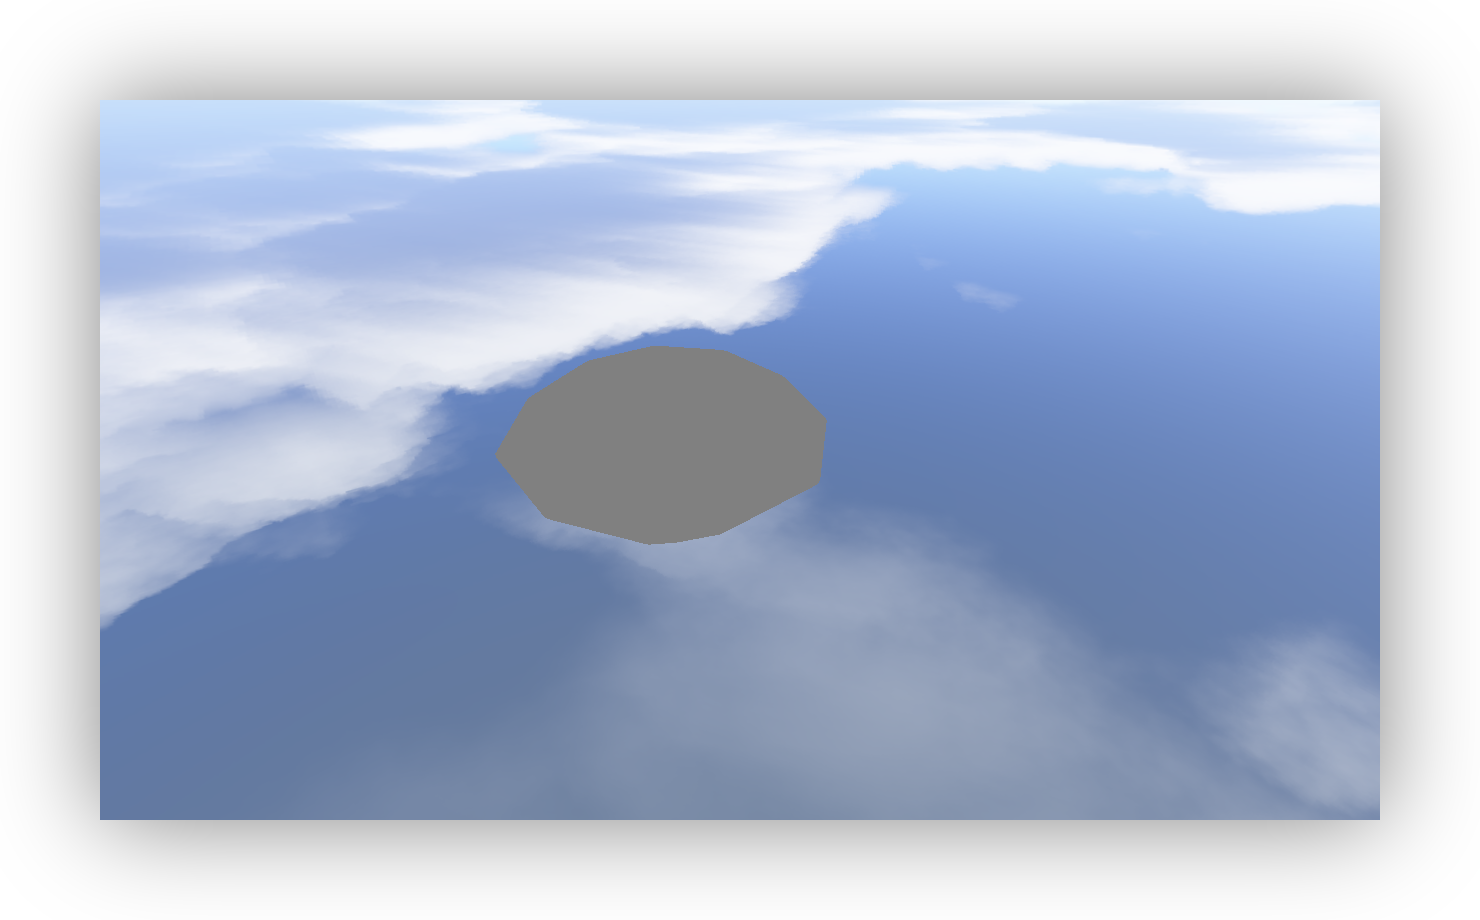
\includegraphics[width=\textwidth]{ssAmbiant}
\caption{Lumière ambiante}
\end{subfigure}\hfill
\begin{subfigure}[b]{0.3\textwidth}
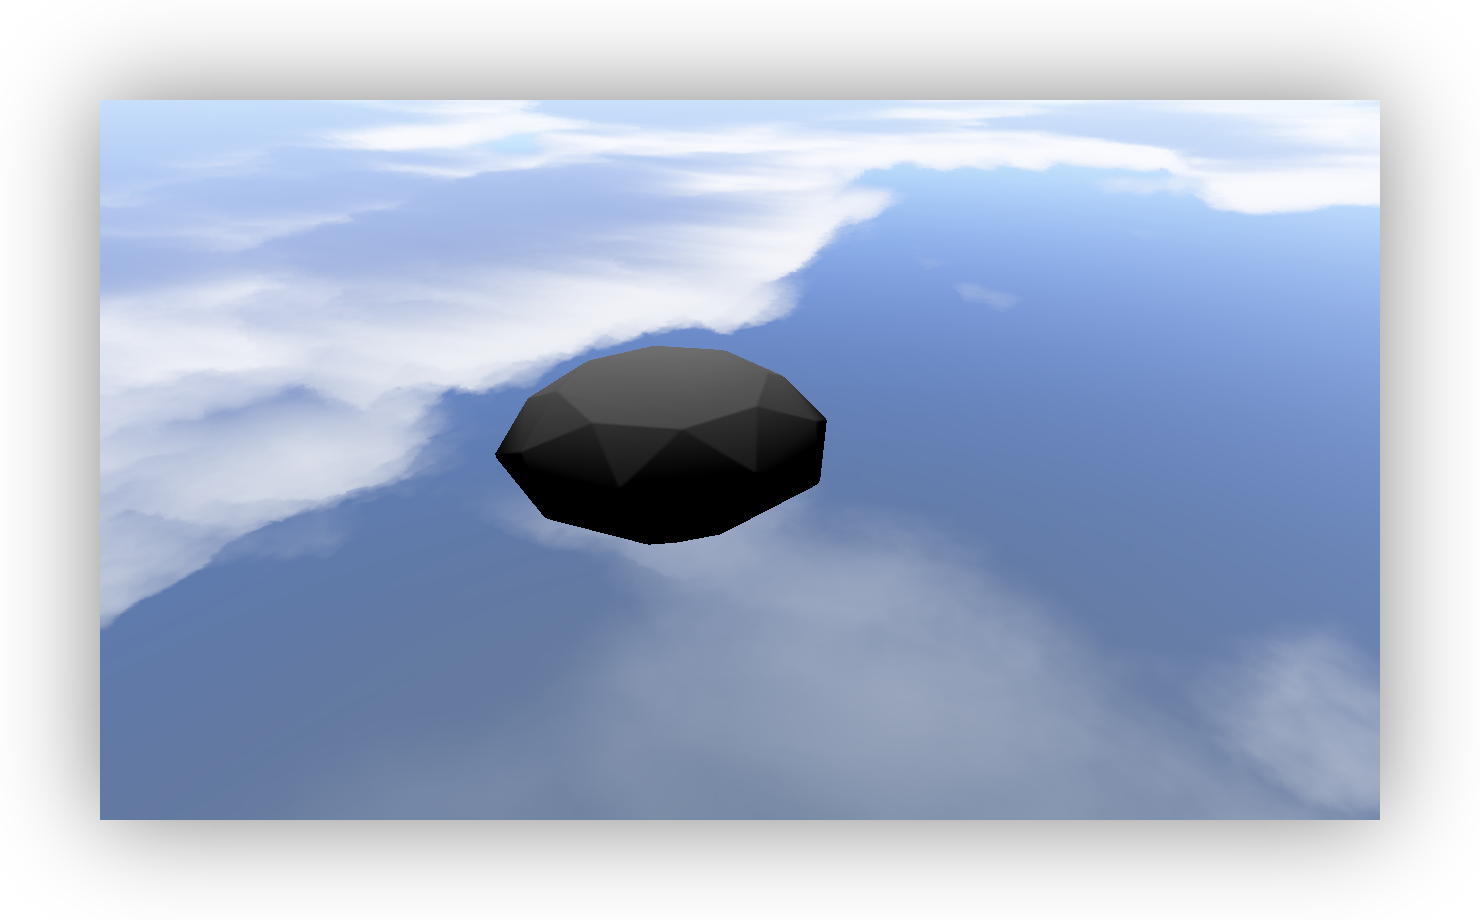
\includegraphics[width=\textwidth]{ssDiffuse}    
\caption{Lumière diffuse}
\end{subfigure}\hfill
\begin{subfigure}[b]{0.3\textwidth}
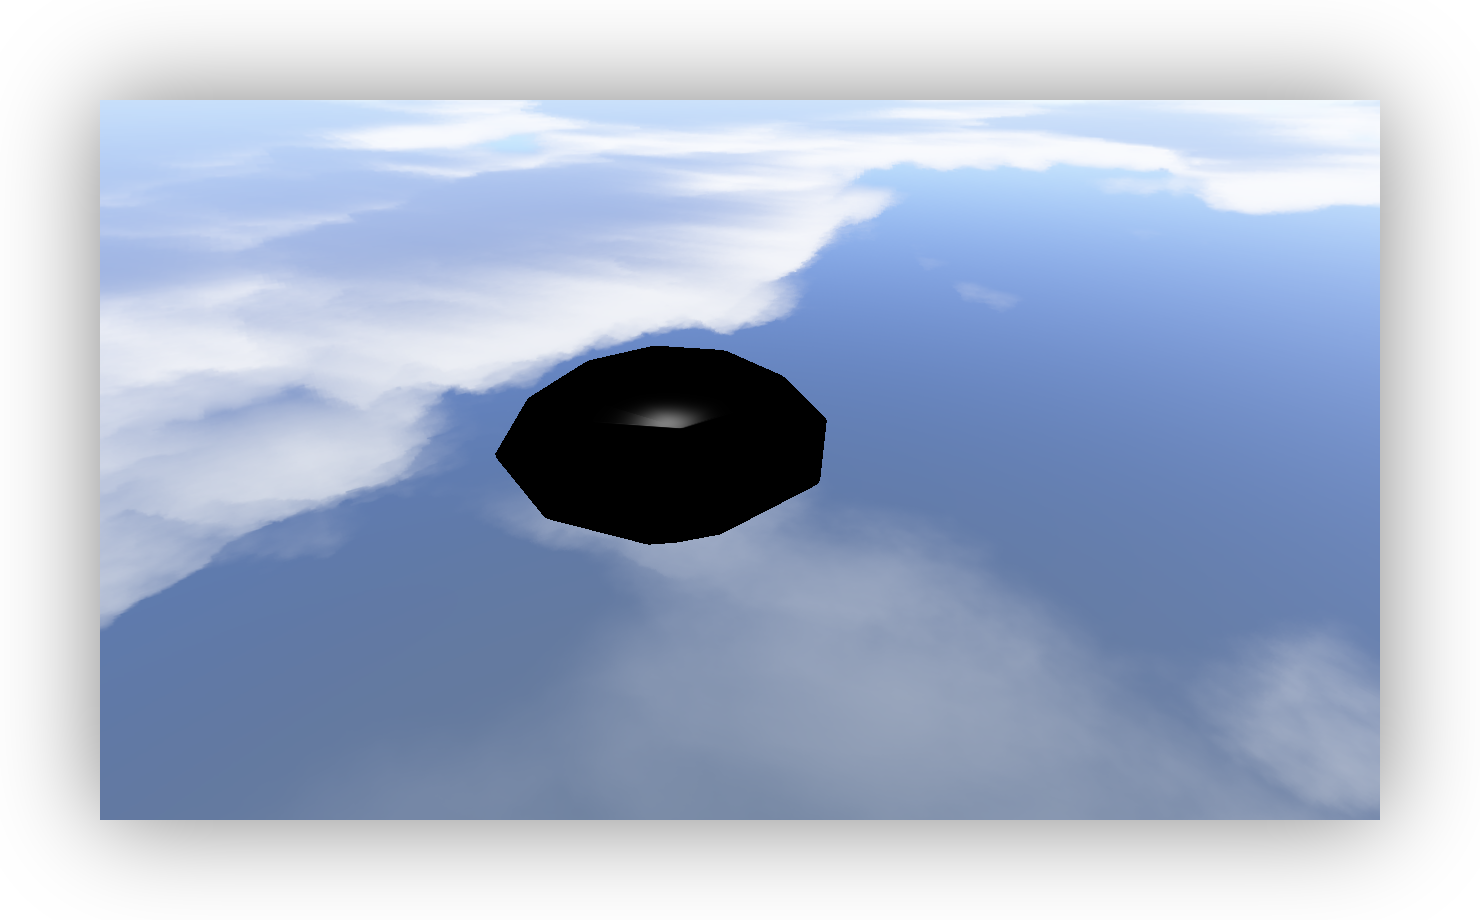
\includegraphics[width=\textwidth]{ssSpecular}    
\caption{Lumière spéculaire}
\end{subfigure}
\end{figure}

\subsubsection{Skybox}

La skybox est un cube avec une taille d'arrête, qui est dessinée tout
 autour de la caméra. En fait, pour suivre la caméra, la partie 3x3 de 
la matrice de vue est utilisée, ce qui a pour effet d'éliminer la
 composante de translation tout en conservant la composante rotation 
qui nous intéresse. Ensuite le cube est dessiné en désactivant l'écriture
 dans le tampon de profondeur, donc n'importe quel objet dessiné après le 
cube apparaîtra à l'écran, même si il se trouve plus loin que les faces
 visibles du cube. Le résultat donne l'impression que la scène se situe
 dans le ciel, avec des nuages que l'on ne peut atteindre.

\paragraph{Réflexion}\mbox{}\\

\begin{wrapfigure}{R}{0.4\textwidth}
\vspace{-35pt}
\begin{centering}
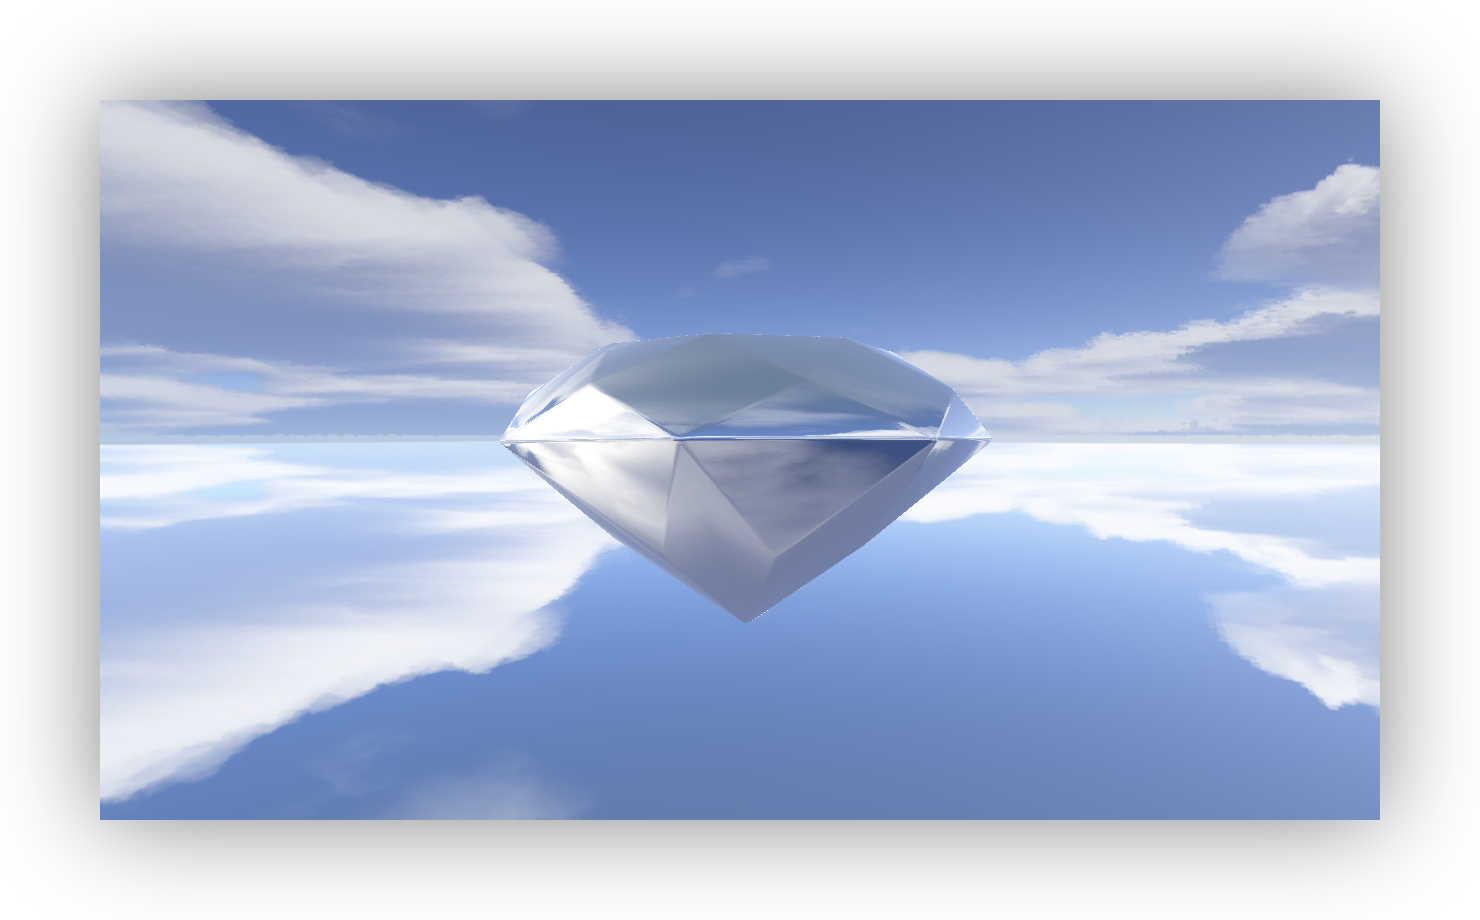
\includegraphics[width=0.4\textwidth]{ssReflect}
\end{centering}
\vspace{-35pt}
\end{wrapfigure}
La réflexion sur les cristaux est simulée par une texture d'environnement 
qui correspond à la skybox qui englobe la scène.
La particularité est que le vecteur de la direction réfléchit correspond 
directement au texel(pixel d'une texture) du cube. On peut donc récupérer
 la couleur facilement et l'afficher sur le cristal, après
l'avoir légèrement mixée avec le reste du fragment (10\%)
La texture est accessible avec 2 coordonnées x et y.

\paragraph{Réfraction}\mbox{}\\

\begin{wrapfigure}{R}{0.4\textwidth}
\vspace{-35pt}
\begin{centering}
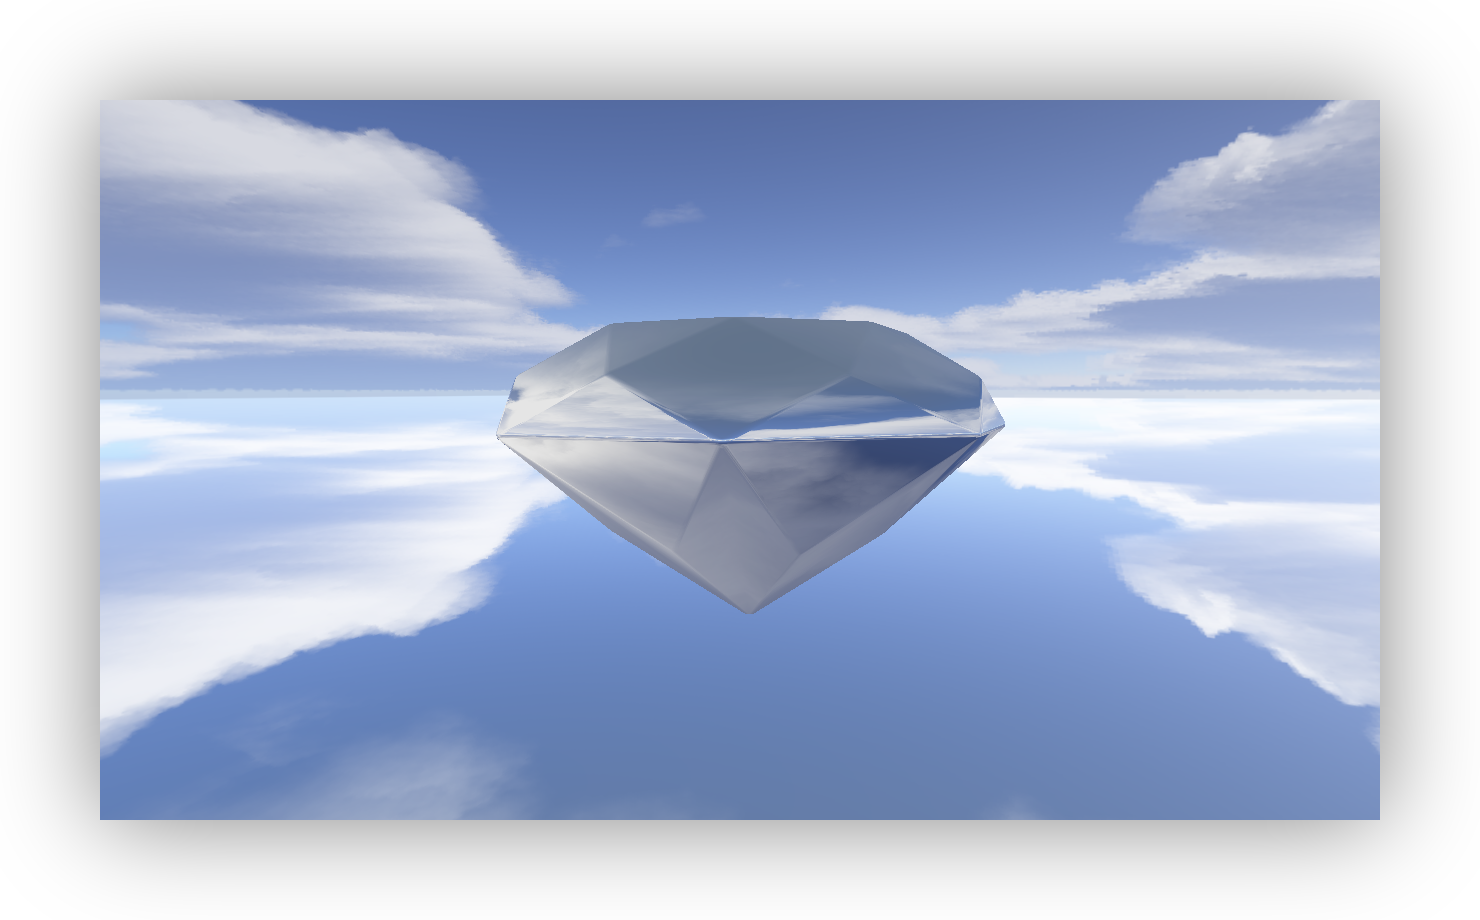
\includegraphics[width=0.4\textwidth]{ssRefract}
\end{centering}
\vspace{-35pt}
\end{wrapfigure}

La réfraction elle, est un peu plus compliquée, le même principe s'adapte, 
sauf qu'au lieu de calculer la réflexion d'un rayon, on calcul la 
déviation avec l'indice de réfraction d'un cristal. La fonction \emph{refract}
 prend en paramètre le rayon de vue, la normale d'incidence et
 l'indice de réfraction. Le rayon réfracté est obtenu selon la
 formule suivante.
\begin{equation*}
R = ir * \vect{Incident} - (ir * \vect{Normale} \times \vect{Incident}) + \sqrt{k}) * \vect{Normale}
\end{equation*}
\pagebreak
\subsubsection{Post-Processing}

\begin{wrapfigure}{R}{0.4\textwidth}
\vspace{-35pt}
\begin{centering}
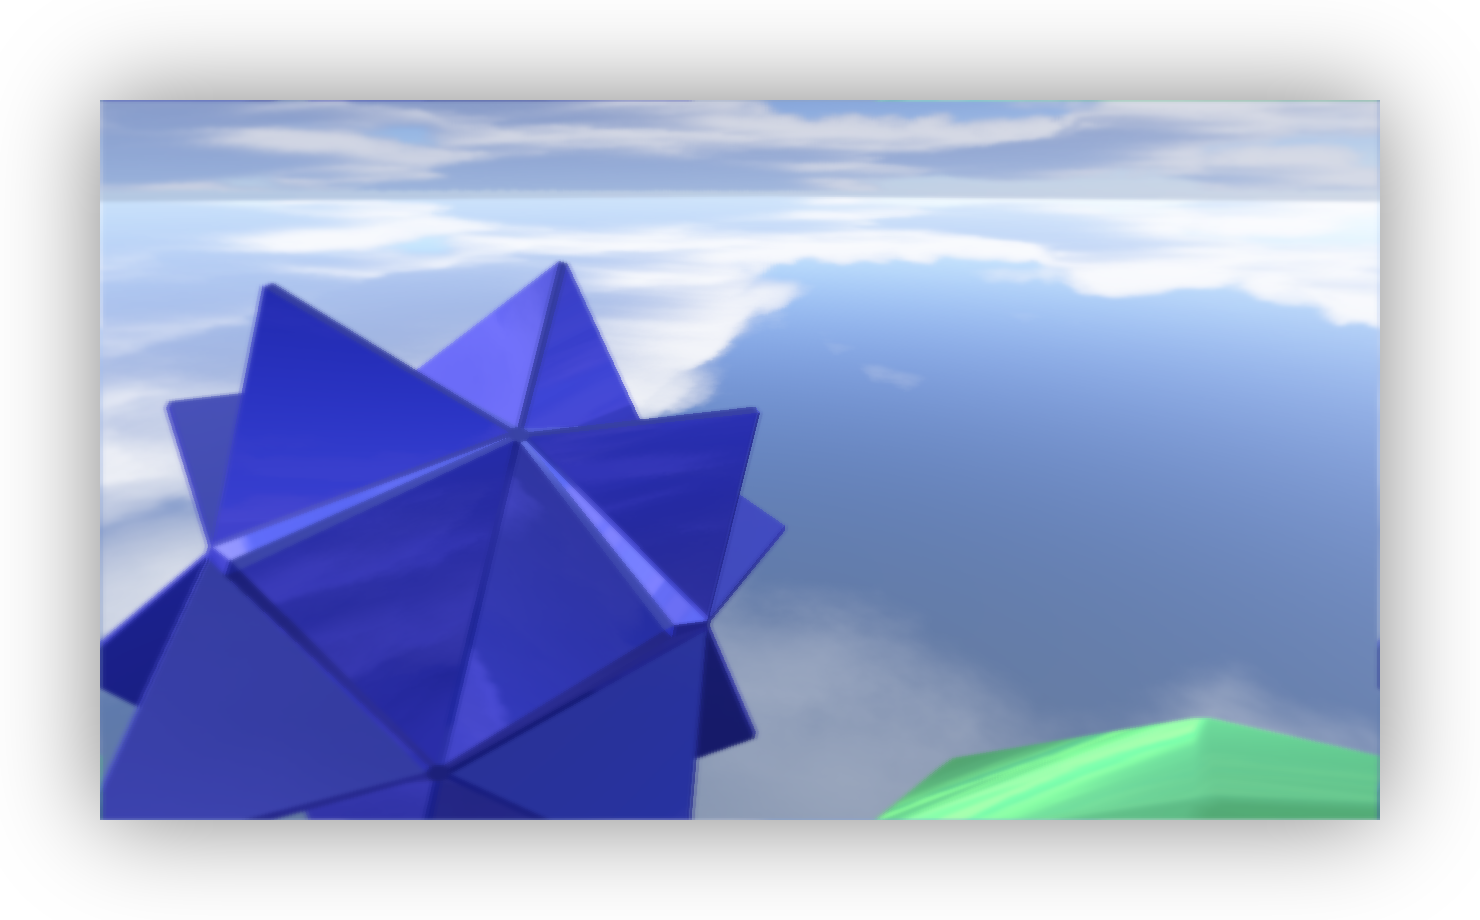
\includegraphics[width=0.4\textwidth]{ssBlur}
\end{centering}
\vspace{-35pt}
\end{wrapfigure}
Le post processing consiste simplement à effectuer un traitement sur
chaque pixel individuel d'une scène, et de ce fait, les implémentations sont
aussi diverses et variées que les effets recherchés. Les shader sont particulièrement
bien adaptés à cet usage, car les algorithmes de traitement d'images étant souvent
inconditionnel, ils peuvent être facilement parallélisé, d'où l'usage important du GPU
dans les logiciels de traitement d'images.
Par exemple, l'inversion d'image consiste simplement à inverser les intensités
des couleurs

\begin{equation*}
CouleurFinale = 1 - Couleur
\end{equation*}

Les effets requérant d'effectuer de l'échantillonnage utilise typiquement
une matrice de convolution, qui détermine les coefficients avec lequel
un pixel influence le résultat final.

Cette matrice de convolution, par exemple, permet d'obtenir une approximation
du flou gaussien.

\begin{equation*}
k =
\begin{bmatrix}
1 & 2 & 1\\
2 & 4 & 2\\
1 & 2 & 1\\
\end{bmatrix}
/ 16
\end{equation*}

Le traitement consiste alors à échantillonner des pixels autour du pixel traité, et de combiner leur valeurs selon cette matrice.
Le shader du fichier basicBlur.glsl utilise cette méthode, si ce n'est qu'en plus
il calcule la distance du pixel par rapport au centre de l'écran pour le brouiller plus
ou moins.


\end{document}
